% ------------------------------------------------------------------------------
% LaTeX template created by
% Iker Algañaraz, May Juarez F., Gastón A. Lozano S., Belén N. Paz
% ------------------------------------------------------------------------------

\documentclass[a4paper,12pt]{article}

% ------------------------------------------------------------------------------
% Packages
% ------------------------------------------------------------------------------
\usepackage{anysize} % Márgenes
\usepackage[hypcap=false, font=small, justification=centering, labelfont=bf]{caption} % Pie de foto/tabla
\usepackage{multicol} % Columnas
\usepackage{amsmath} % Fórmulas matemáticas
\usepackage{amssymb} % Símbolos matemáticos
\usepackage{amsfonts} % Font matemática
\usepackage[utf8]{inputenc} % Facilitar la escritura en español
\usepackage{xcolor} % Color del texto
\usepackage{graphicx} % Figuras
\usepackage[spanish,es-tabla]{babel} % Tipografía del idioma
\usepackage{booktabs} % Separación en tablas
\usepackage{multirow} % Multirow en tablas
\usepackage{hyperref} % Refs como hyperlinks
%\usepackage{biblatex} % Bibliografía automática a partir de base bib

%\usepackage{array}
%\usepackage{verbatim}% Comentarios multilinea
%\usepackage{siunitx} % Unidades del sistema internacional
%\usepackage{fancyhdr} % Personalizar encabezado y pie de pagina
%\usepackage{longtable} % Tablas largas
%\usepackage{blindtext} % Lore ipsum
%\usepackage{soul} % Subrayar
%\usepackage{grffile}
%\usepackage{mathrsfs}

% ------------------------------------------------------------------------------
% Config
% ------------------------------------------------------------------------------
\newenvironment{Figure}
  {\par\medskip\noindent\minipage{\linewidth}}
  {\endminipage\par\medskip}

\providecommand{\abs}[1]{\lvert#1\rvert} % Valor absoluto

\marginsize{2cm}{2cm}{1cm}{2cm} % pkg: anysize

\graphicspath{{./Fotos/}} % pkg: graphicx

\setlength\columnsep{18pt}
\setlength\parskip{4pt} \setlength\parindent{0in}

\title{ Interferencia \\ 
\medskip \large Universidad Nacional de Tucumán}
\author{May Juarez Ferriol}
\date{}

% ------------------------------------------------------------------------------
% Document
% ------------------------------------------------------------------------------
\begin{document}

\maketitle

\section*{Interferencia}

    Llamamos interferencia al efecto que se produce al combinar dos o más ondas de luz en un punto del espacio. Este efecto es muy complicado de observar por lo chicas que son las longitudes de onda que estamos analizando (entre $4 \times 10^{-7}\ m$ y $7 \times 10^{-7}\ m$ aproximadamente). Sin embargo, hay dos condiciones que facilitan mucho la visualización de esté fenómeno, y es que las fuentes que generen esas ondas sean coherentes, es decir que \emph{la relación entre las fases de las dos ondas no cambie con el tiempo}, y que las ondas tengan longitudes de onda idénticas.

    Decimos que la interferencia es constructiva si la intensidad de la combinación es mayor que las intensidades individuales. Mientras que decimos que la intereferencia es destructiva si la intensidad total es menor que las intensidades individuales.

\section*{Patrón de interferencia}

    La intensidad del patrón de interferencia es de acuerdo al de la figura \ref{fig:Int_Interferencia}.

    \begin{Figure}
        \centering
        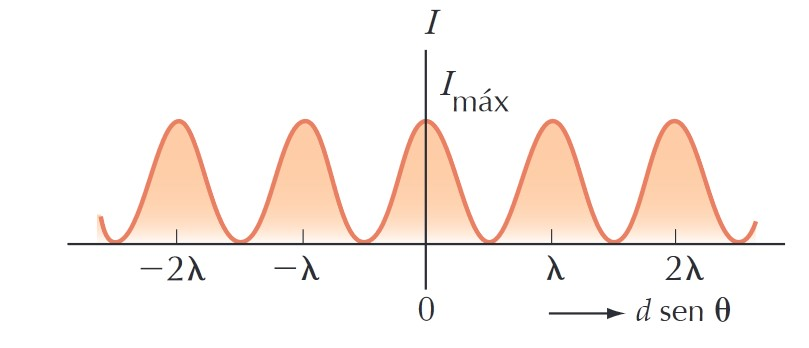
\includegraphics[width=0.75\linewidth]{Intensidad_interferencia.jpg}
        \captionof{figure}{Intensidades de un patrón de interferencia de doble rendija}
        \label{fig:Int_Interferencia}
    \end{Figure}

    En la realidad, todo patrón de interferencia se verá modulado por un patrón de difracción, por lo que la intensidad que se observaría en realidad es como la de la imágen \ref{fig: patronInterferenciaDifraccion}.

    \begin{Figure}
        \centering
        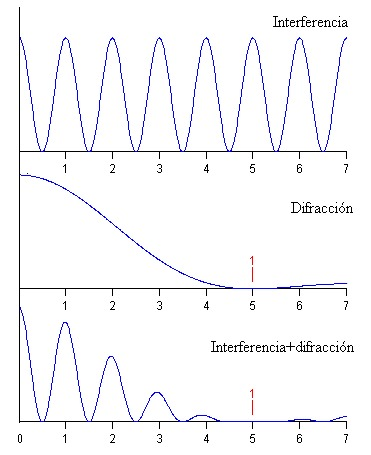
\includegraphics[width=0.5\linewidth]{patronInterferenciaDifraccion.jpg}
        \captionof{figure}{Intensidades de un patrón de interferencia de doble rendija modulado por un patrón de difracción}
        \label{fig: patronInterferenciaDifraccion}
    \end{Figure}

\section*{¿Por qué se observan colores cuando se iluminan ranuras con luz blanca?}

    Cuando la luz blanca incide sobre una serie de ranuras delgadas, como las de una rejilla o una lámina delgada, puede ocurrir un fenómeno conocido como difracción.

    En el contexto de la difracción de luz blanca a través de ranuras, el fenómeno clave es que la luz blanca está compuesta por diferentes longitudes de onda, que corresponden a diferentes colores. Cada longitud de onda se desvía de manera ligeramente diferente al pasar por las ranuras, debido a las diferencias en la difracción para cada color.

    Este proceso de difracción separa las diferentes longitudes de onda y dispersa los colores, creando un patrón de colores en la región donde la luz difractada se proyecta. Este fenómeno es conocido como el espectro de difracción.

    El espectro de difracción generado suele tener un patrón característico, con colores más dispersos en los bordes y colores más centrados en el centro. El ángulo de difracción y la separación entre las ranuras afectan la distribución de los colores en el patrón de difracción.

    \begin{Figure}
        \centering
        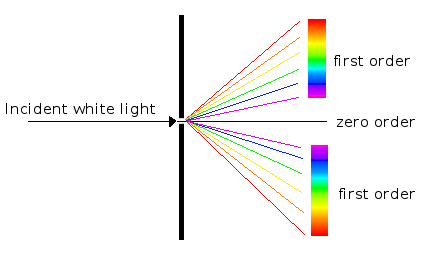
\includegraphics[width=0.6\linewidth]{Diffraction.png}
        \captionof{figure}{Difracción de luz blanca}
        \label{fig: patronDifraccion}
    \end{Figure}

\section*{El experimento de la doble rendija de Young}

    El experimento de Young, realizado por el científico británico Thomas Young en 1801, es un experimento clásico que proporcionó evidencia clave para la teoría ondulatoria de la luz. El experimento demostró el fenómeno de interferencia de la luz, respaldando la idea de que la luz se comporta como una onda.

    \begin{Figure}
        \centering
        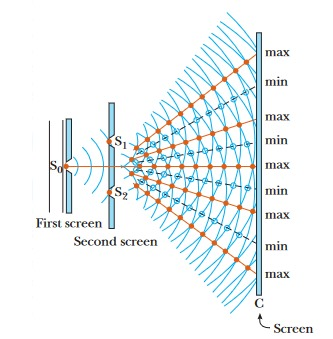
\includegraphics[width=0.5\linewidth]{Young.jpg}
        \captionof{figure}{Diagrama del experimento de doble rendija de Young}
        \label{fig: Young}
    \end{Figure}

    La luz es incidente en una primera pantalla que contiene una rendija $S_0$. Las ondas de luz que salen de esta rendija llegan a la segunda pantalla con dos ranuras estrechas y paralelas $S_1$ y $S_2$. Estas ranuras actuan como dos fuentes de ondas coherentes, ya que las ondas que llegan a cada una vienen del mismo frente de onda y por lo tanto siempre están en fase.

    Después de pasar a través de las ranuras, la luz incidía en una pantalla colocada a cierta distancia. En la pantalla, se observaba un patrón de interferencia, con franjas claras y oscuras.

    \begin{Figure}
        \centering
        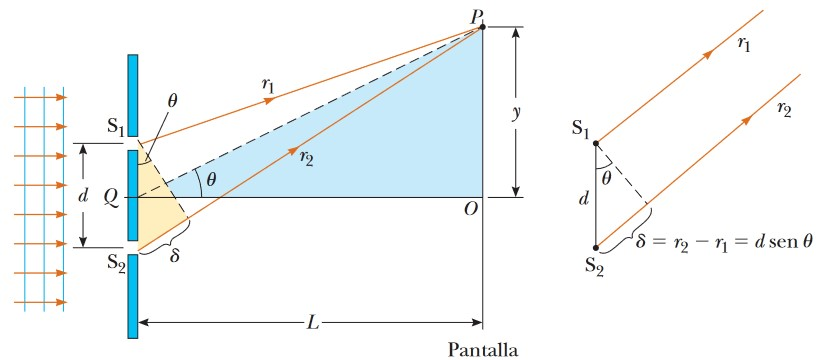
\includegraphics[width=0.75\linewidth]{DeduccionInterferencia.jpg}
        \captionof{figure}{Interferencia para un arreglo de dos rendijas que actuan como fuentes coherentes}
        \label{fig:DeduccionInterferencia}
    \end{Figure}
    
    Supongamos dos fuentes de luz, $S_1$ y $S_2$, separadas por una distancia $d$ tal que $d \approx \lambda$, que producen ondas viajeras simultaneamente y a la misma frecuencia. A un punto $P$ de una pantalla a una distancia $L$ medida perpendicularmente, se obtienen una distancia $r_1$ y $r_2$ a cada una de las fuentes. Vemos que en este arreglo obtenemos máximos de interferencia, es decir interferencia constructiva donde la suma neta de los campos eléctricos (o magnéticos) de ambas ondas emitidas desde $S_1$ y $S_2$ sea mayor a 0. En esos puntos se cumple la ecuación \ref{eq:Deduccion_constructiva}.

    \begin{equation}
        r_2 - r_1 =  m\lambda,\ m=0,\pm1, \pm2,...
        \label{eq:Deduccion_constructiva}
    \end{equation}

    Si ahora utilizamos una aproximación con angulos $\theta$, encontramos que $ r_2 - r_1 = d \sin\theta $. Entonces reemplazando en la expresión \ref{eq:Deduccion_constructiva}, obtenemos la ecuación \ref{eq:InterConstruc}. Si trabajamos con la aproximación de angulos pequeños ($\theta_{max} \approx 13^o$ ), podemos aproximar las expresiones a la tangente del ángulo $\theta$.

    \begin{equation}
        \tan \theta \approx \sin \theta =  \frac{\lambda}{d}\ m
        \label{eq:InterConstruc}
    \end{equation}

    \begin{equation}
        y =  \frac{\lambda L}{d}\ m
        \label{eq: InterConstruc}
    \end{equation}

\section*{Cuestionarios}

    \begin{Figure}
        \centering
        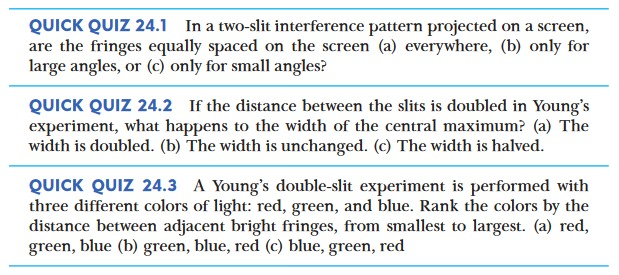
\includegraphics[width=0.8\linewidth]{quiz.jpg}
        \label{fig: cuestionarios}
    \end{Figure}

    \textbf{Quick Quiz 24.1.-} (c) Es necesario que se cumpla la aproximación de ángulos pequeños.

    \textbf{Quick Quiz 24.2.-} (c) Como se puede ver en la ecuación (\ref{eq: InterConstruc}), los tamaños en la pantalla son inversamente proporcionales a la separación entre las rendijas.
    
    \textbf{Quick Quiz 24.3.-} (c) Como se puede ver en la figura \ref{fig: patronDifraccion}, el orden es azul, verde y rojo. Es decir, de mayor longitud de onda a menor longitud de onda.

\begin{thebibliography}{99}

\bibitem{} R. A. Serway, C. Vuille. \emph{College Physics}, 11th ed. (Cengage, Australia, 2018)

\bibitem{} R. A. Serway, J. W. Jewett. \emph{Physics for Scientists and Engineers with Modern Physics}, 10th ed. (Cengage, Australia, 2017)

\bibitem{} H. D. Young, R. A. Freedman. \emph{Sears and Zemansky's University Physics: with Modern Physics}, 14th ed. (Pearson, Boston, 2016)

\end{thebibliography}

\end{document}

% ------------------------------------------------------------------------------
% Common references and examples
% ------------------------------------------------------------------------------
% 
% ---------------------------
% Bibliography
% ---------------------------
% \bibitem{} Sears, Zemansky. \emph{Física universitaria}, vol. 2, 14th ed. Pearson Education, 2018.
% \bibitem{} Hecht, Zajac. \emph{Óptica}, 4th ed. Pearson Education, 2003.
% \bibitem{} Serway, Jewett. \emph{Physics for Scientists and Engineers}, vol. 2, 6th ed. Brooks Cole, 2004.
% \bibitem{} Jenkins, White. \emph{Fundamentos de óptica}, 3th ed. Aguilar S.A., 1964.
%
% ---------------------------
% Tables
% ---------------------------
% \begin{Figure}
%     \centering
%
%     \begin{tabular}{c|c}
%         \toprule
%          & \textit{...} \\
%          & \textit{[]} \\
%         \midrule
%         ... & \multirow{2}{*}{$(... \pm ...)$} \\
%         ... & \\
%         ... & \multirow{2}{*}{$(... \pm ...)$} \\
%         ... & \\ \hline
%         ... & $(... \pm ...)$ \\
%         ... & $(... \pm ...)$ \\
%         \bottomrule
%     \end{tabular}
%
%     \captionof{table}{}
%     \label{tab:}
% \end{Figure}
%
% \begin{Figure}
%     \centering
%
%     \begin{tabular}{cc}
%         \toprule
%         \textit{\textbf{... []}} & \textit{\textbf{$... []}}\\
%         \midrule
%         $... \pm ...$ & $... \pm ...$ \\
%         $... \pm ...$ & $... \pm ...$ \\
%         \bottomrule
%     \end{tabular}
%
%     \captionof{table}{}
%     \label{tab:}
% \end{Figure}
%
% ---------------------------
% Figures
% ---------------------------
% \begin{Figure}
%     \centering
%     \includegraphics[width=1\linewidth]{.jpg}
%     \captionof{figure}{}
%     \label{fig:}
% \end{Figure}
%
% ---------------------------
% Equations
% ---------------------------
% \begin{equation}
%     \label{eq:}
%     ...
% \end{equation}